\chapter{Dezvoltarea soluției}\label{ch:4dezvoltareaSolutiei}

	Acest capitol conține o prezentarea detaliată a modului în care a fost implementat proiectul. Voi face referiri atât la partea harware, cât și la partea software. 

\section{Specificarea cerințelor}
	...

\section{Arhitectura sistemului}

\begin{figure}[H]
   	\centering
    	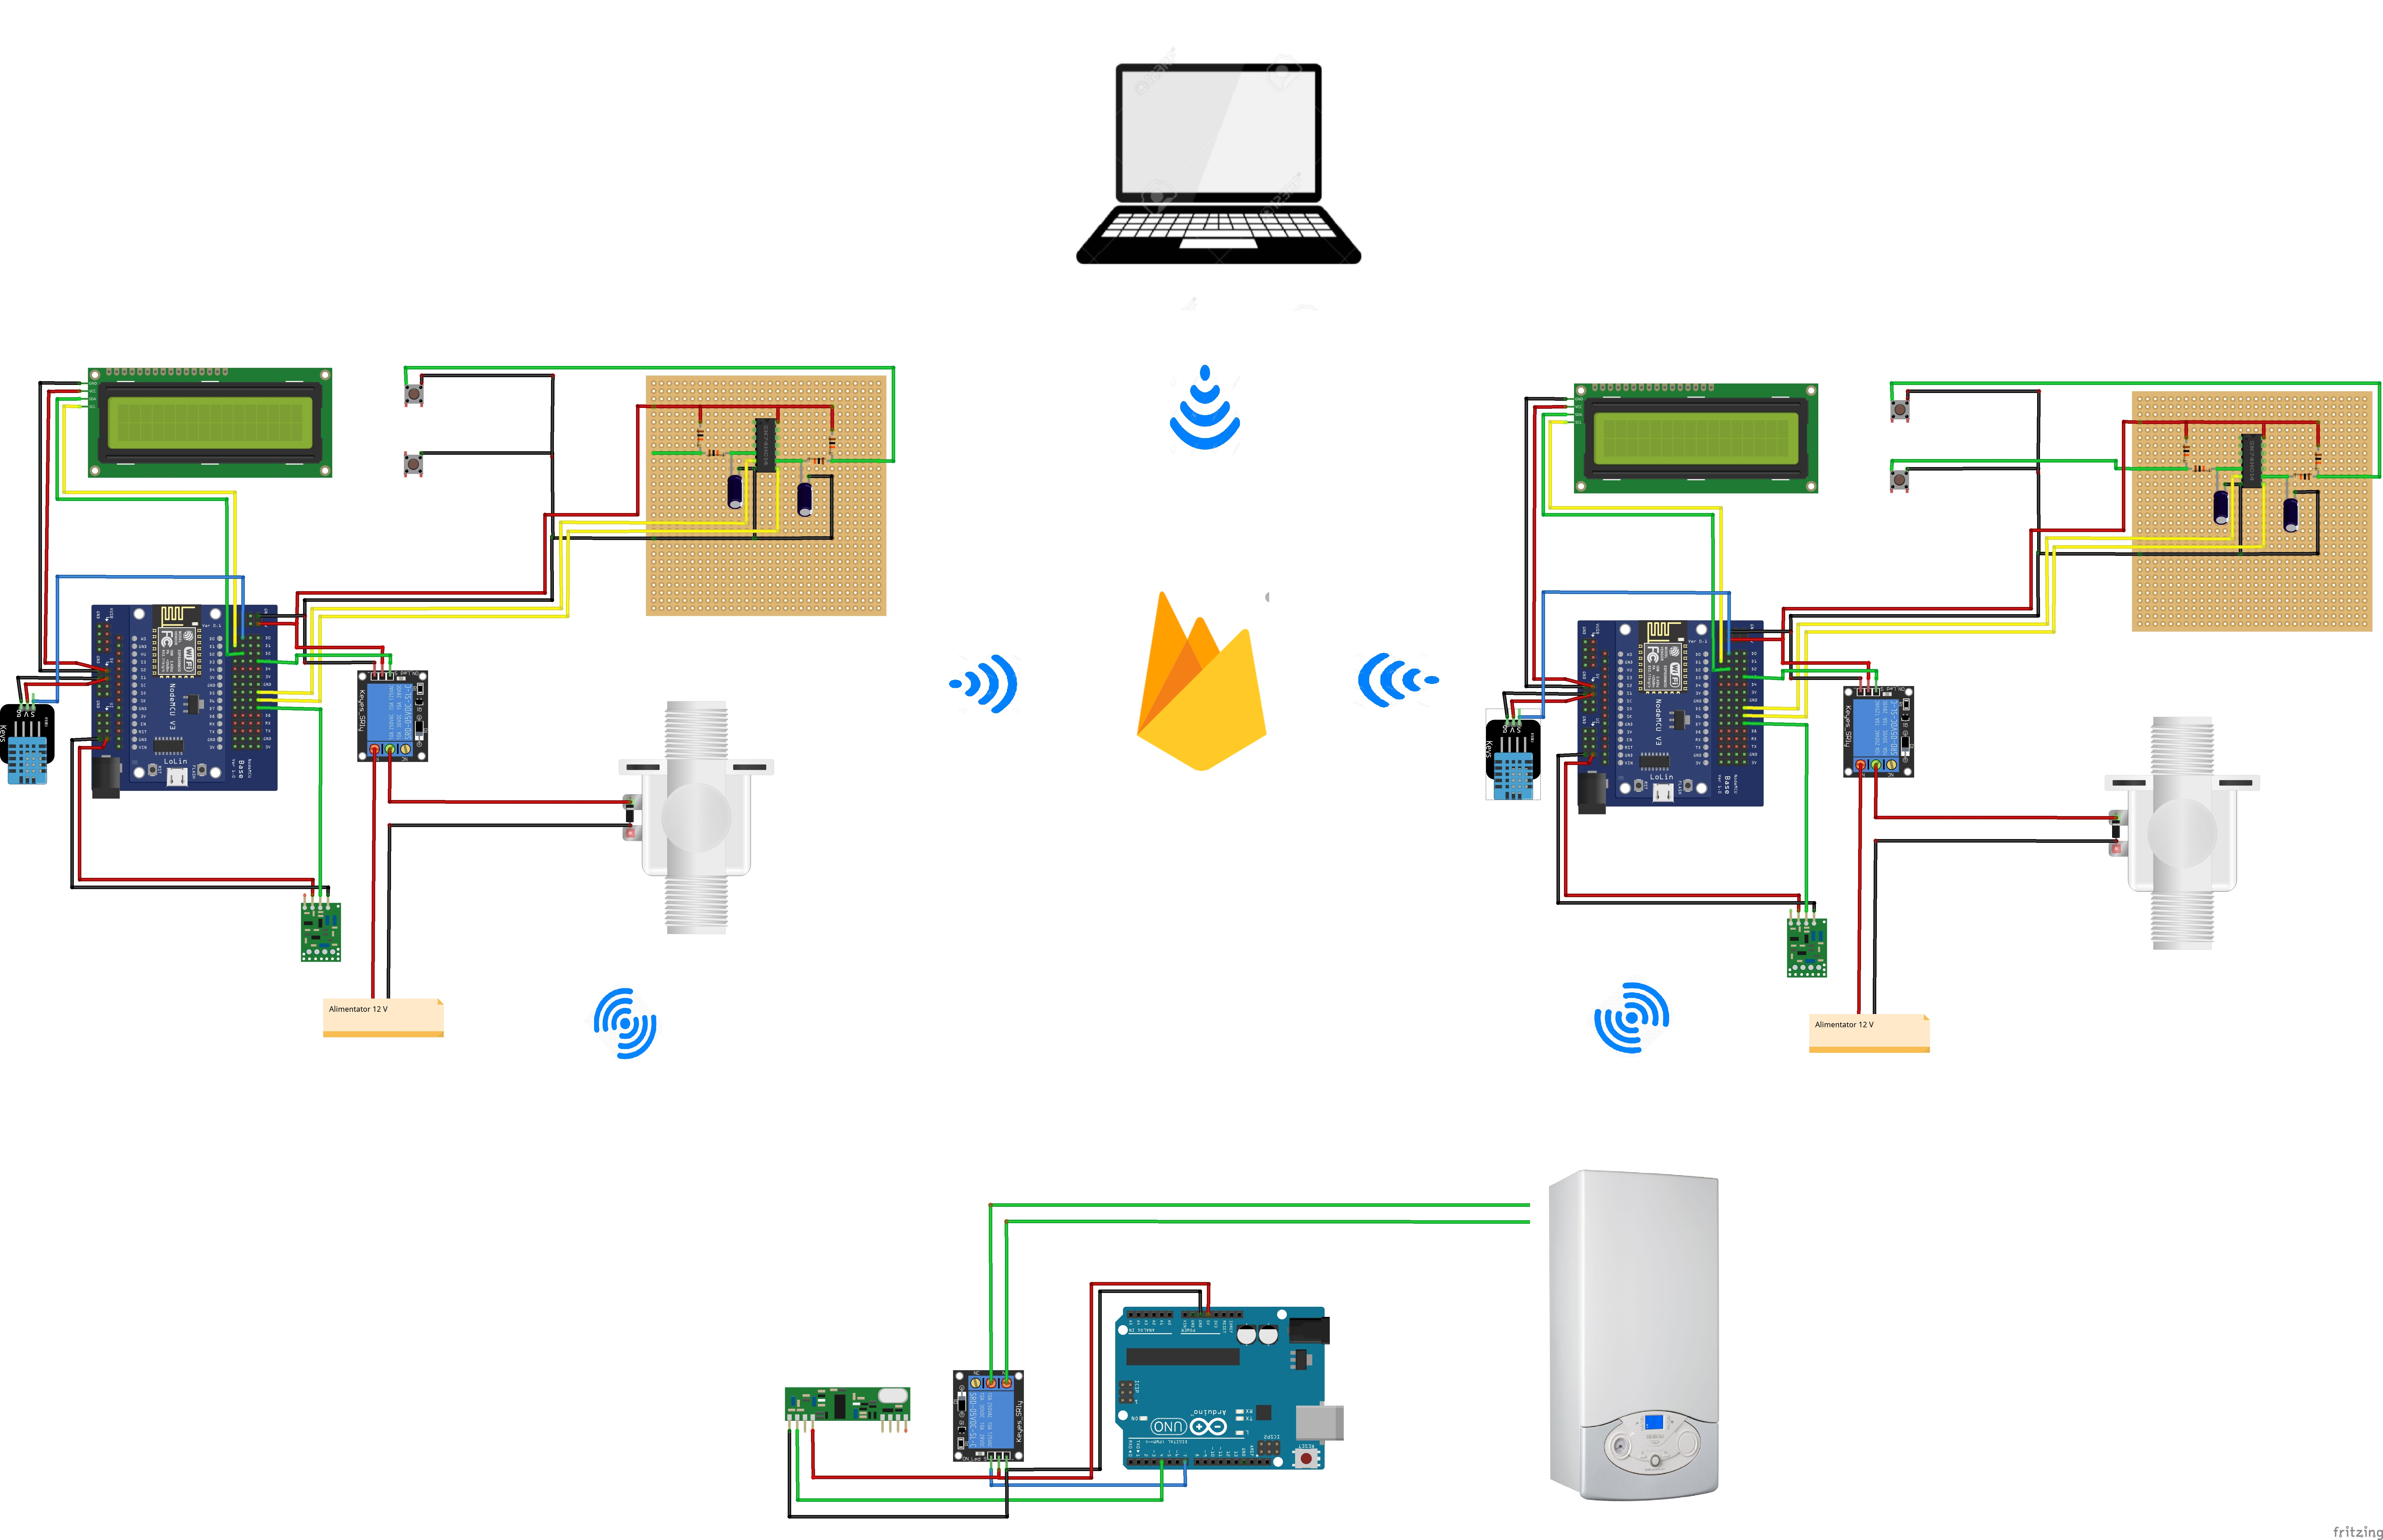
\includegraphics[width=1\textwidth]{ArhitecturaSistemului.jpg}
	\caption{Arhitectura sistemului}
\end{figure}

	Sistemul a fost conceput pentru un apartament cu două camere, însă poate fi extins pentru un număr mai mare de încăperi. La nivel macro, este format din trei module, câte un modul senzor pentru fiecare cameră și un modul de control, montat în apropierea centralei termice.

	Modulul senzor prezintă o complexitate mai mare, este alcătuit din mai multe componente și îndeplinește o serie de funcționalități. Preia informații precum: temperatura și umiditatea și le trimite în baza de date. În continuare, aceste valori sunt afișate utilizând aplicația web, făcând posibilă monitorizarea parametrilor ambientali. De asemenea, are acces la temperatura setată, iar in funcție de aceasta și de temperatura curentă din cameră controlează electrovalva și trimite comandă de oprire sau pornire a centralei. Un alt rol esențial pe care îl îndeplinește modulul, este de a face posibilă setarea unei valori a temperaturii ce urmează să fie menținută în cameră.

	Modulul de control este de o complexitate redusă. Primește comenzi de la modulele senzor, iar în funcție de acestea controlează centrala. Modulul se folosește de logică de tip "SAU", dacă cel puțin un modul senzor trimite comandă de pornire, atunci centrala termică trebuie să înceapă ciclul de încălzire.

	Transferul de date între modulele senzor și modulul de control se face prin intermediul undelor radio, 433 MHz. Placuțele ESP8266 se folosesc de unde Wi-Fi, 2.4 GHz, pentru a se conecta la router.

\subsection{Modulul senzor}

\begin{figure}[H]
   	\centering
    	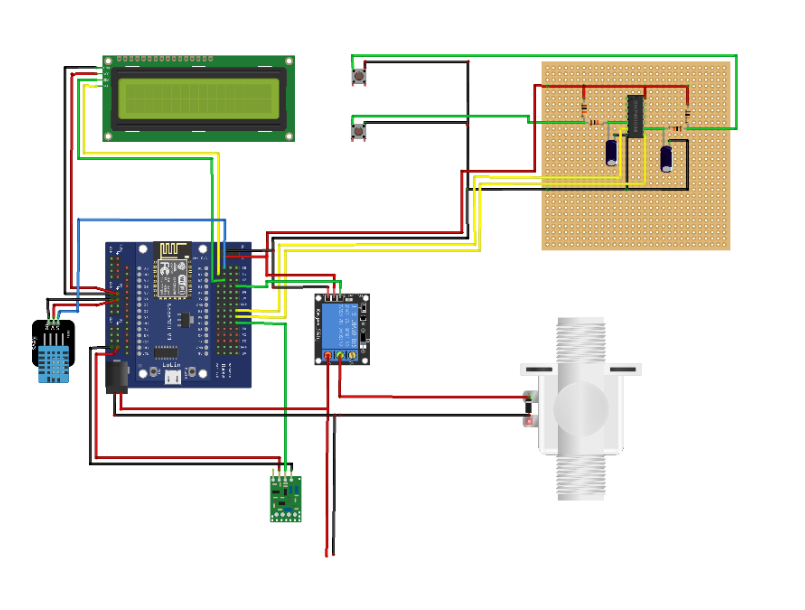
\includegraphics[width=1\textwidth]{ModulSenzor.png}
	\caption{Arhitectura sistemului}
\end{figure}	

	Este format din următoarele componente:
	\begin{itemize}
		\setlength{\itemindent}{2em}
			\itemsep0em
			\item Modul WiFi NodeMCU
			\item Placă de bază pentru NodeMCU
			\item LCD
			\item Senzor de temperatură și umiditate
			\item Releu
			\item Butoane
			\item Transmițător RF
			\item Electrovalvă
			\item Invertor de semnal
			\item Rezistență
			\item Condensator
			\item Alimentator 12 volți
	\end{itemize}

	Componenta principală din acest ansamblu este modulul wireless. Se conectează prin WiFi la un punct de acces al rețelei, router-ul în cazul proiectului prezentat, și face transfer de date cu baza de date utilizată. Acesta pune la dispoziție o serie de pini pentru a putea conecta diverse componente auxiliare. 
	
	Pinul D0 este utilizat pentru a conecta pinul de date de la senzorul de temperatură și umiditate.

	Pinii D1 și D2 se conectează la pinii SCL și SDA pentru a face posibil transferul de date prin protocolul de comunicație $I^2C$.

	Pinul D3 se conectează la pinul IN al releului și are rolul de a controla închiderea sau deschiderea releului, iar pinii D5 și D6 sunt rezervați pentru butoane. 

	Pinul D7 transferă date la pinul de date al transmițătorului RF. 

\vspace{1em}

	Placa de bază pentru modulul WiFi are două roluri esențiale în crearea circuitului. Acesta facilitează felul în care se poate alimenta plăcuța wireless, punând la dispoziție o mufă de alimentare care poate fi conectată la alimentatoare ce furnizează tensiuni între 6 și 24 de volți. Prin intermediul unui regulator de tensiune va aduce tensiunea de alimentare a modulului WiFi până la 5 volți, prevenind orice posibilitate de supraalimentare. Astfel, placa de bază pune la dispoziție pini ce oferă tensiuni de ieșire de 3.3 volti, 5 volți și o serie de pini ce sunt conectați direct la mufa de alimentare și furnizează voltaj egal cu cel dat de alimentator. De asemenea, oferă pentru fiecare pin al modulului ESP8266 încă 4 pini corespondenți, fapt ce reprezintă un avantaj când vine vorba de conectarea unor componente auxiliare.

\vspace{1em}

	Pentru a putea afișa temperatura curentă din cameră și temperatura setată, se folosește un display. Transferul de date între LCD și modulul WiFi, la care este conectat, se face prin intermediul protocolului de comunicație $I^2C$. S-a ales acest protocol deoarece reduce considerabil numărul de fire necesare pentru conectarea și alimentarea LCD-ului, în acest caz fiind necesare doar 4. Prin urmare, display-ul pune la dispoziție următorii pini:  VCC, GND, SDA și SCL.

\vspace{1em}

	Senzorul de temperatură și umiditate se ...protocol de comunicație

\vspace{1em}

	Releul este conectat la modulul wireless și este controlat de acesta prin pinul IN. Rolul releului este de întrerupător în circuitul electric format din electrovalvă și alimentator.

\vspace{1em}

	Sunt prezente două butoane ce permit modificarea temperaturii setate. Butonul de sus incrementează temperatura și se conectează la pinul D5 al modului WiFi, iar butonul de jos decrementează valoarea temperaturii și se conectează la pinul D6.

\vspace{1em}

	Transmițătorul RF prezintă 3 pini: VCC, GND și DATA. Pinii VCC și GND se conectează la o sursă de tensiune, ieșirile de 12 volți oferite de placa de bază NodeMCU. Pinul de date se conectează la pinul digital D7 al modulului wireless și face posibil transferul de date între acestea. În continuare, datele vor fi transferate la receptorul de tip RF, montat pe modulul de control.  

\vspace{1em}

	Electrovlava se montează pe returul caloriferelor și este responsabilă cu închiderea sau deschiderea circuitului de apă din calorifer. Releul este cel care întrerupe, sau nu, alimentarea electrică a electrovalvei

\vspace{1em}

	Invertorul de semnal, rezistența și condensatorul sunt componente electrice pe care le-am utilizat pentru a filtra semnalul provenit de la buton.  

\subsection{Modulul de control}